%
% This document is free; you can redistribute it and/or modify
% it under the terms of the GNU General Public License as published by
% the Free Software Foundation; either version 2 of the License, or
% (at your option) any later version.
%
% This document is distributed in the hope that it will be useful, but
% WITHOUT ANY WARRANTY; without even the implied warranty of
% MERCHANTABILITY or FITNESS FOR A PARTICULAR PURPOSE.  See the GNU
% General Public License for more details.
%
% You should have received a copy of the GNU General Public License
% along with this document; if not, write to the Free Software
% Foundation, Inc., 51 Franklin Street, Fifth Floor, Boston, MA
% 02110-1301, USA.
%
% Author: Bertoli Marco
%
\chapter{JSIM}
\label{cha:jsim}
\section{Simulation engine architecture}
\subsection{General architecture}
All simulator engine classes are included in \texttt{jmt.engine}
package: its structure is shown in \autoref{fig:jsim:package}.

\begin{figure}[htbp]
    \begin{center}
        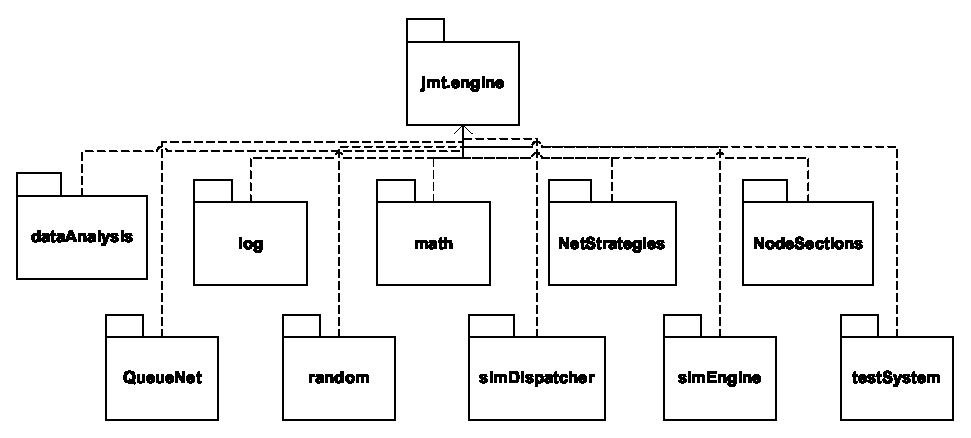
\includegraphics[scale=.65]{img/jsim/Package_engine}
    \end{center}
    \caption{\texttt{jmt.engine} package structure}
    \label{fig:jsim:package}
\end{figure}

This package does not directly includes any classes but is divided
in more \emph{subpackages} with different functionalities which are
briefly described:
\begin{description*}
    \item[simEngine:] this is the \emph{kernel} of the simulator,
    used to manage the entire system, the \emph{entities} in the system
    (i.e. stations) and the \emph{discrete event calendar} which is the
    base of the entire simulator.
    \item[QueueNet:] this package is directly placed upon
    \texttt{simEngine} and is used to introduce basic components of
    queueing network theory. Customer classes are introduced along
    with the node entity which will be subclassed by every type of
    service center. Its interfaces are used to abstract from the
    \texttt{simEngine} data structures and provide a 


    \emph{entity} into a

    � il secondo package in ordine di importanza: si appoggia sul cuore
    del simulatore, mascherandone i dettagli di basso livello e controllandone lo stato.
    \item[NodeSections:] contiene le classi che definiscono tutti i possibili
    componenti delle stazioni di servizio, ad esempio code, serventi, router e
    delay.
    \item[NetStrategies:] contiene tutte le politiche ammissibili per la coda,
    per il servizio e per il routing.
    \item[dataAnalysis:] � il package che gestisce il calcolo degli intervalli
    di confidenza all'interno della simulazione.
    \item[random:] contiene il generatore di numeri casuali e le classi che
    implementano le diverse distribuzioni statistiche. Come generatore di numeri casuali,
    il jSIM utilizza il Mersenne Twister (si vedano la Sezione~\ref{sec:generatoreNumeriCasuali}
    e \cite{Mersenne}).
    \item[log:] contiene la classe e il file di configurazione che servono per loggare
    messaggi di debug, informazioni, warning, errori durante il funzionamento del jSIM.
    Si appoggia sul package esterno Log4J (si veda \cite{log4j}).
    \item[math:] contiene le classi di supporto per le operazioni
    matematiche, ad esempio distribuzioni statistiche e FFT.
    \item[simDispatcher:] contiene le classi necessarie per eseguire simulazioni passando
    come parametro il file XML contenente la descrizione del
    modello.
    \item[testSystem:] permette di eseguire una serie di test per valicare i risultati del
    simulatore. La generazione dei modelli e il confronto dei risultati del simulatore con
    quelli dei metodi esatti avvengono in modo automatico.\end{description*}
